% !TeX spellcheck = it_IT
\documentclass[10pt,a4paper]{article}

\usepackage[utf8]{inputenc}
\usepackage[T1]{fontenc}	
\usepackage[italian]{babel}
\usepackage{amsmath}
\usepackage{amsfonts}
\usepackage{amssymb}
\usepackage{graphicx}

\usepackage[left=2cm,right=2cm,top=2cm,bottom=2cm]{geometry}
\geometry{a4paper}

\usepackage{booktabs} % for much better looking tables
\usepackage{verbatim}
\usepackage{subfig} % make it possible to include more than one captioned figure/table in a single 

\usepackage{fancyhdr} % This should be set AFTER setting up the page geometry
\pagestyle{fancy} % options: empty , plain , fancy
\renewcommand{\headrulewidth}{0pt} % customise the layout...
\lhead{}\chead{}\rhead{}
\lfoot{}\cfoot{\thepage}\rfoot{}

%%% SECTION TITLE APPEARANCE
\usepackage{sectsty}
%\allsectionsfont{\sffamily\mdseries\upshape} % (See the fntguide.pdf for font help)
% (This matches ConTeXt defaults)

% pacchetti che mi fanno schifo ma uso lo stesso (Bob è scemo, ma anche Ale...)
\usepackage[cdot, thickqspace, squaren]{SIunits}
% il miglior pacchetto che potessi desiderare
\usepackage{float}
% macro che mi piacciono
\def\code#1{\texttt{#1}}


\title{Esercitazione 7: Amplificatore operazionale, usi non lineari}

\author{Gruppo BE \\ Alessandro Candido, Roberto Ribatti}
\date{\today}
\begin{document}
\maketitle

\section{Scopo e strumentazione}

\section{Discriminatore}
Si è montato il circuito in \figurename{~\ref{circuito_discriminatore}} e se ne è studiata la risposta a segnali sinusoidali di frequenza e intensità variabili. In \figurename{~\ref{fig:discriminator}} è mostrato il comportamento ad una frequenza di $\sim \unit{1}{k\hertz}$ ed una tensione di ingresso di $\sim\unit{4}{\volt}$, è visibile l'onda sinusoidale in ingresso e l'onda quadra generata in uscita dall' op-amp. Poiché l'op-amp è usato in modalità invertente il comportamento è paragonabile ad un circuito logico NOT.

\begin{figure}[H]
	\begin{minipage}{0.49\textwidth}
		\centering
		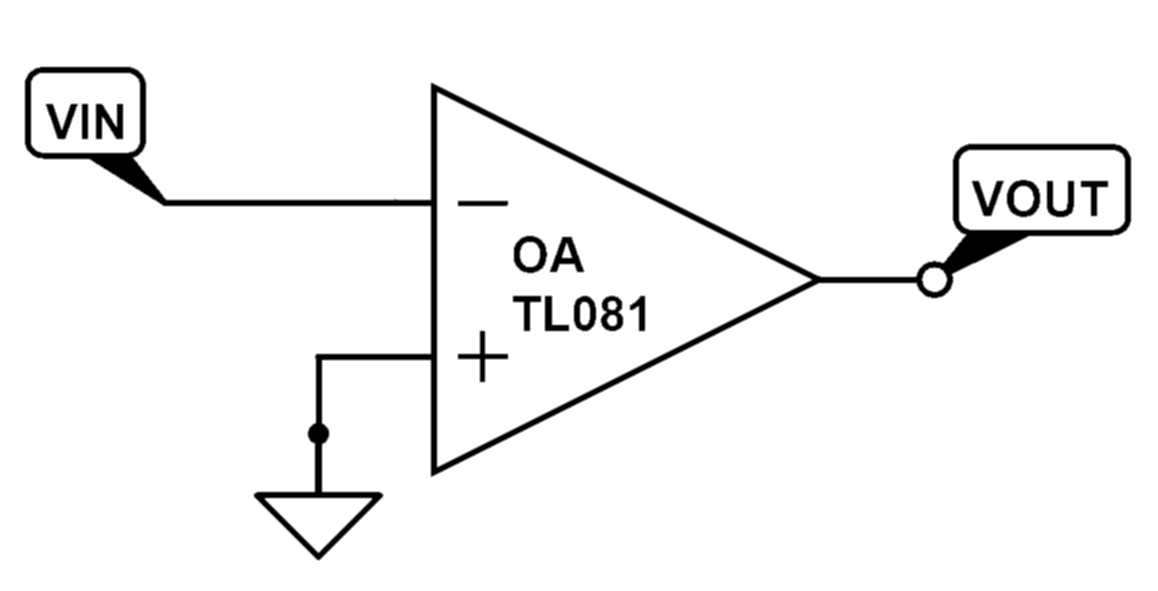
\includegraphics[width=0.7\textwidth]{../circuiti/discriminatore.jpg}
		\caption{Schema del circuito discriminatore}
		\label{circuito_discriminatore}
	\end{minipage}
	\begin{minipage}{0.49\textwidth}
		\centering
		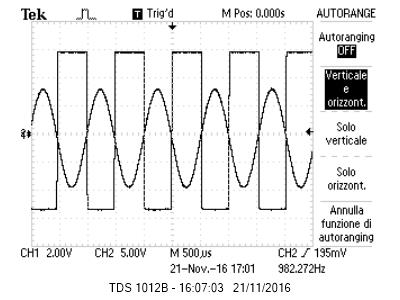
\includegraphics[width=0.9\textwidth]{../oscilloscopio/discriminator.jpg}
		\caption{Risposta del circuito discriminatore}
		\label{fig:discriminator}
	\end{minipage}
\end{figure}

\subsection{Misura della tensione di offset}
Si è proceduto a studiare in maggior dettaglio il punto di zero-crossing e a misurare la tensione di offset $V_{OS}$, ovvero la tensione del segnale sinusoidale $V_{IN}$ nell'istante in cui il segnale in output attraversa lo zero ($V_{OUT}=0$). In \figurename{~\ref{fig:vos}} è visibile il punto di zero crossing e il risultato della misura: $V_{OS} = \unit{150 \pm 5}{\milli\volt}$.

\begin{figure}[H]
	\centering
	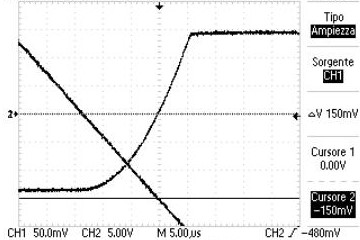
\includegraphics[width=0.45\textwidth]{../oscilloscopio/Vos.jpg}
	\caption{Zoom sul punto di zero-crossing e misura di $V_{OS}$}
	\label{fig:vos}
\end{figure}

\subsection{Conservazione prodotto GBW}
Per elevate frequenze è atteso, per la conservazione del prodotto guadagno-banda che il guadagno dell'op-amp diminuisca. Per piccoli segnali in ingresso e alte frequenze è possibile quindi che il segnale in output non arrivi a saturazione e sia visibile come un onda sinusoidale.

In \figurename{~\ref{fig:GBW}} è visibile la risposta del circuito ad un segnale di $\sim\unit{100}{k\hertz}$ e un'intensità $V_{IN}= \unit{156 \pm 5}{\milli\volt}$ e come atteso il segnale è sinusoidale.

Si è misurata la risposta a varie frequenze a parità di tensione di input (sempre rimanendo in remime lineare), i dati raccolti sono riportati in appendice in \tablename{~\ref{tab:GBW}}. Si è fittata la conservazione del prodotto banda guadagno $Af_h$, i grafici e i risultati del fit sono riportati di seguito (a e b sono rispettivamente coefficiente angolare e intercetta):

\begin{figure}[H]
	\begin{minipage}{0.28\textwidth}
		\centering
		\begin{tabular}{l}
			$a = \unit{-19.5 \pm 0.7}{\deci\bel / decade}$ \\
			$b = \unit{125 \pm 4}{\deci \bel}$ \\
			$\chi^2 / ndof = 1.9/3$\\
			$corr(a,b) = -0.9987$\\
			$Af_h = \unit{2.57+/-0.16}{\mega\hertz}$
		\end{tabular}
	\end{minipage}
	\begin{minipage}{0.75\textwidth}
		\centering
		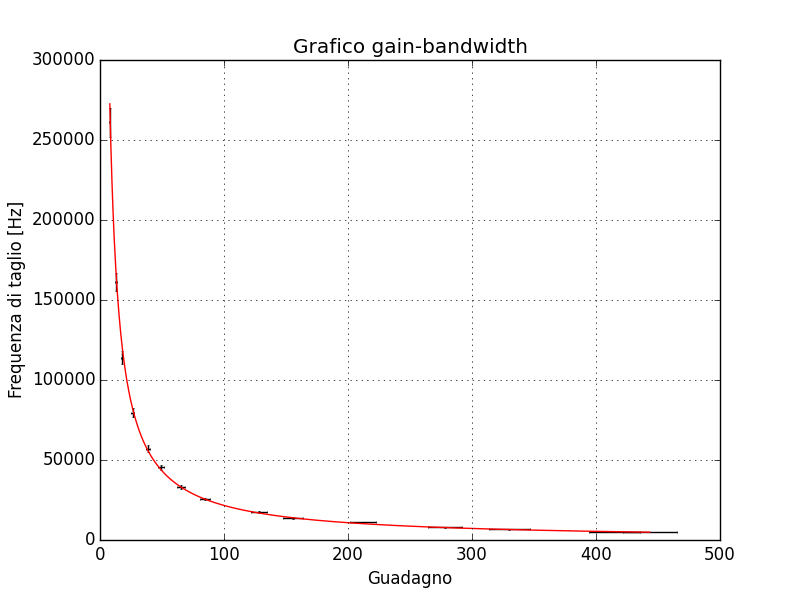
\includegraphics[width=0.95\textwidth]{../grafici/fit_gain_bandwidth.pdf}
		\caption{Dati e fit della conservazione del GBW}
		\label{}
	\end{minipage}
\end{figure}

\begin{figure}[H]
	\begin{minipage}{0.49\textwidth}
	\centering
	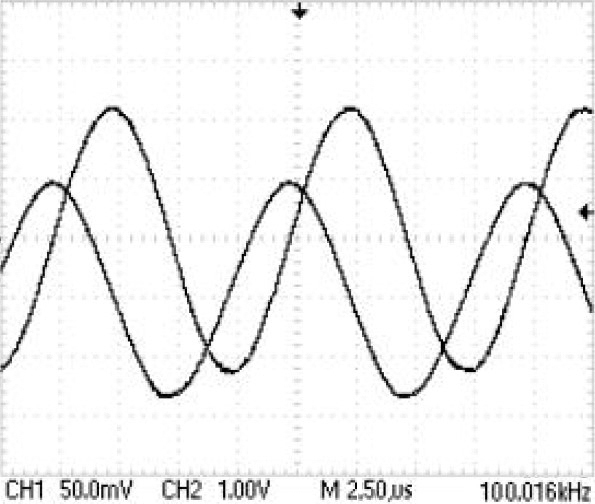
\includegraphics[width=0.85\textwidth]{../oscilloscopio/discriminatore_GBW.jpg}
	\caption{Regime di linearità (alte frequenze e piccolo segnale)}
	\label{fig:GBW}
	\end{minipage}
	\begin{minipage}{0.49\textwidth}
	\centering
	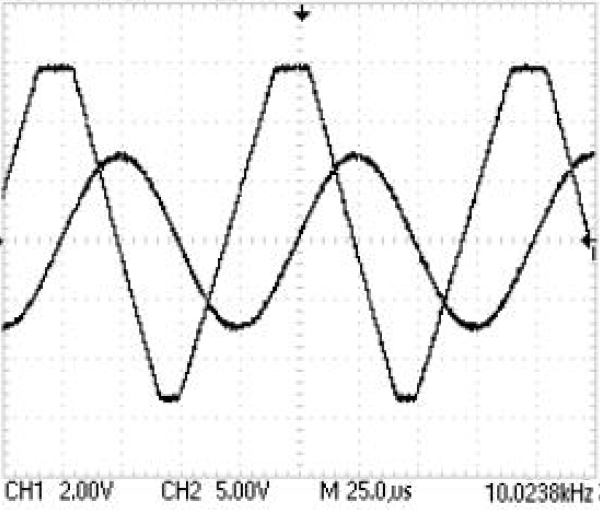
\includegraphics[width=0.85\textwidth]{../oscilloscopio/discriminator_slewrate.jpg}
	\caption{Deformazione dell'onda quadra dovuta allo slew-rate (medie frequenze, grande segnale)}
	\label{fig:slewrate_razzista}
	\end{minipage}
\end{figure}

\subsection{Slew rate}
Per frequenze medio/alte e grandi segnali lo slew-rate produce una notevole distorsione dell'onda quadra limitanto la velocità di salita/discesa del segnale. Gli effetti dello slew-rate sulla risposta del circuito sono chiari in \figurename{~\ref{fig:slewrate_razzista}}. Si è misurata la velocità di discesa del segnale, il valore trovato è stato $\unit{13.4 \pm 0.4}{\volt /\micro\second}$, compatibile con il valore di $\unit{13}{\volt / \micro\second}$ riportato nel datasheet.

\section{Amplificatore di carica}

Si è montato il circuito in \figurename{~\ref{circuio_ampli}} con i seguenti valori dei componenti:

\begin{figure}[H]
	\begin{minipage}{0.3\textwidth}
		\centering
		\begin{tabular}{l}
			$C_1 = \unit{21.0 \pm 0.9}{\nano\farad}$  \\ 
			$C_T = \unit{0.99 \pm 0.05}{\nano\farad}$ \\
			$C_F = \unit{1.00 \pm 0.05}{\nano\farad}$ \\
			$R_1 = \unit{99.1 \pm 0.9}{k\ohm}$  \\
			$R_2 = \unit{98.8 \pm 0.9}{\ohm}$
		\end{tabular}
	\end{minipage}
	\begin{minipage}{0.7\textwidth}
		\centering
		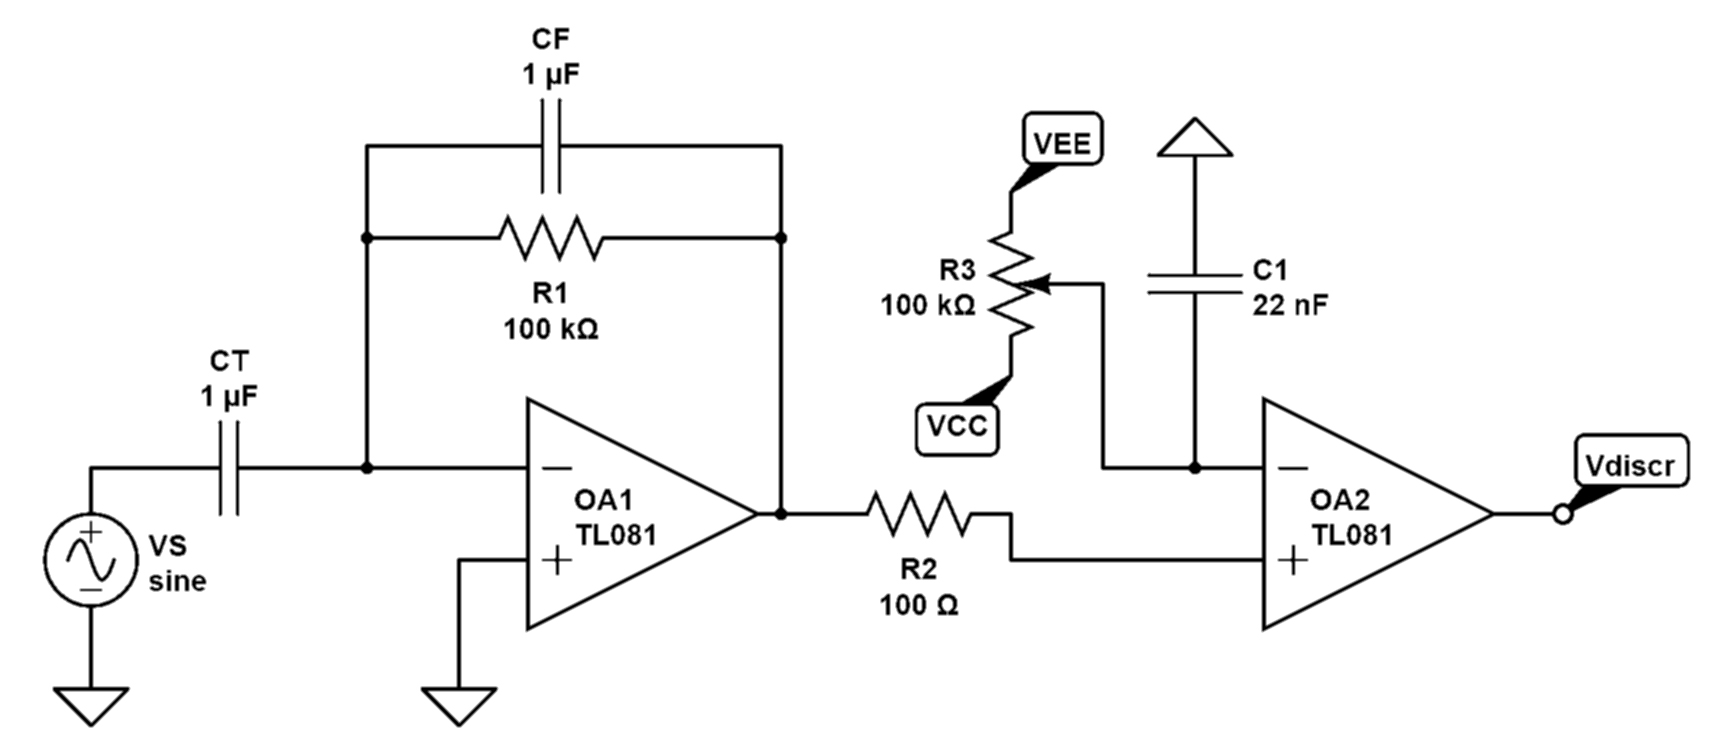
\includegraphics[width=\textwidth]{../circuiti/charge_amplifier.jpg}
		\caption{Schema del circuito amplificatore di carica}
		\label{circuio_ampli}
	\end{minipage}
\end{figure}

Si è misurata la durata del segnale in uscita al variare dell'intensità del segnale in ingresso, i dati raccolti sono riportati in \tablename{~\ref{tab:V_t}}.
Dalla teoria sappiamo che $t = \tau \cdot ln(V_{IN}/V_0)$, dove $V_0$ è la tensione di soglia fissata nel discriminatore e $\tau = R_1 \cdot C_F$.

Si sono fittate le misure eseguite, i grafici e i risultati del fit sono di seguito riportanti.

\begin{figure}[H]
	\begin{minipage}{0.28\textwidth}
		\centering
		\begin{tabular}{l}
			$\tau = \unit{99.7 \pm 0.6}{\micro\second}$ \\
			$V_0 = \unit{272 \pm 5}{\milli \volt}$ \\
			$\chi^2 / ndof = 7.8/11$\\
			$corr(\tau,V_0) = -0.956$\\
		\end{tabular}
	\end{minipage}
	\begin{minipage}{0.75\textwidth}
		\centering
		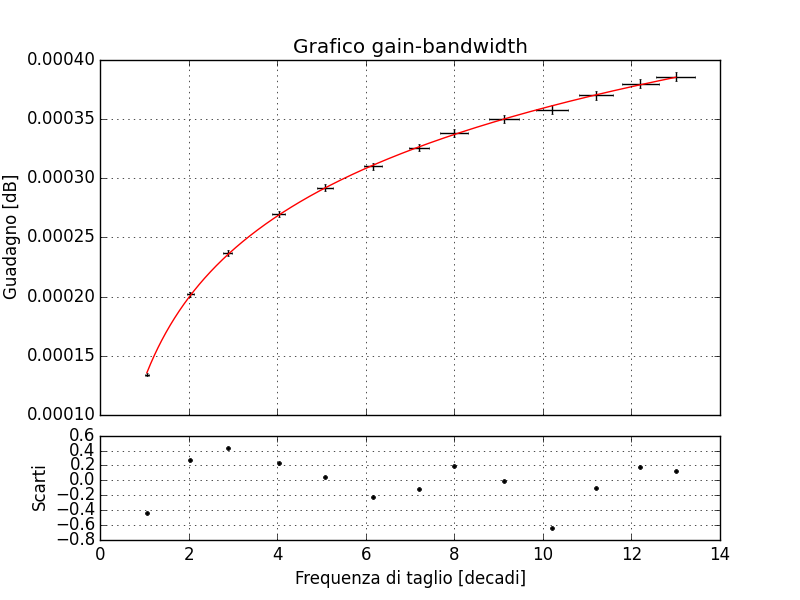
\includegraphics[width=\textwidth]{../grafici/fit_V_t.pdf}
		\caption{Dati e fit sul circuito amplificatore di carica}
		\label{}
	\end{minipage}
\end{figure}

I risultati trovati sono in ottimo accordo con quelli attesi, cioè $\tau^{exp} = \unit{98 \pm 5}{\micro\second}$ e $V_0 = \unit{271 \pm 2}{\milli\volt}.

\section{Trigger di Schmitt}

\section{Multivibratore astabile}

\pagebreak
\section{Appendice: Dati acquisiti}
Si riportano qui le tabelle dei dati usati per i fit e i grafici.

\centering
\begin{figure}[h!]
	\begin{minipage}[t]{0.49\textwidth}
		\centering
		\resizebox{0.7\textwidth}{!}{
		\input{../tabelle/tab_gain_bandwidth.txt}}
		\captionof{table}{Conservazione GBW}
		\label{tab:GBW}
	\end{minipage}
	\begin{minipage}[t]{0.5\textwidth}
		\centering
		\resizebox{0.7\textwidth}{!}{
		\input{../tabelle/tab_V_t.txt}}
		\captionof{table}{Tensione input vs TOT}
		\label{tab:V_t}
	\end{minipage}
\end{figure}




\end{document}
